\documentclass[fleqn,9pt,xcolor=dvipsnames]{beamer}

%========================================
% Packages
%========================================

\usepackage{etex}

\usepackage[]{mypackBeamer}

\usepackage{pgfplots}

\usepackage[absolute,overlay]{textpos}



%========================================
% Commands
%========================================

\usepackage{mycommands}

%========================================
% More Layout (Beamer Special)
%========================================

\DefineNamedColor{named}{mycol}{cmyk}{0.35,1,0.7,0.1}
\DefineNamedColor{named}{myblue}{cmyk}{0.5,0,0.8,0.2}
\DefineNamedColor{named}{mygray}{cmyk}{0.05,0.05,0.05,0.05}
\DefineNamedColor{named}{mygraylight}{cmyk}{0.017,0.017,0.017,0.017}


\usecolortheme[named=mycol]{structure}

\useoutertheme[compress,subsection=false]{miniframes}

\setbeamercolor{background canvas}{bg=white}

\setbeamercolor{lower separation line head}{bg=mygray}


% \usecolortheme[named=Gray]{structure}

% \setbeamercolor{title}{fg=Blue}

%\setbeamercolor{structure}{fg=Brown}
%\setbeamercolor{normal text}{fg=Brown}
%\setbeamercolor{section in head/foot}{bg=gray!40}
%%\setbeamercolor{lower separation line head}{bg=black!40}
%\setbeamercolor*{frametitle}{fg=Black,bg=gray!40}
%\setbeamercolor*{block body}{fg=Brown,bg=gray!00}
%\setbeamercolor*{block title}{fg=Black,bg=gray!40}
 

% Switch of shadows of boxes
\setbeamertemplate{blocks}[default]

% Frame numbers in footer
\setbeamertemplate{footline}[frame number]

% See-through preview for uncovered
\setbeamercovered{transparent}

% Switch off navigation panel at bottom right
\beamertemplatenavigationsymbolsempty

% Change Style for itemize markers
% Options are ball, circle, rectangle and default (=triangle)
\setbeamertemplate{items}[circle] 




\setcounter{tocdepth}{1}

% Use bullets in enumerates and TOC
\setbeamertemplate{enumerate item}[circle]

% Set color for enumerate/TOC bullets to white
\setbeamercolor*{item projected}{fg=Black,bg=gray!00}

%========================================
% Special this document
%========================================

\renewcommand{\markdef}[1]{{\color{mycol}{#1}}}
\newcommand{\myblue}[1]{{\color{myblue}{#1}}}
\newcommand{\mygray}[1]{{\color{gray}{#1}}}
\newcommand{\mycol}[1]{{\color{mycol}{#1}}}

\newcommand{\mycomment}[1]{\hfill {\mygray{(#1)}}}
\newcommand{\mycom}[1]{\hfill {\mygray{#1}}}

\newcommand{\slideFN}[1]{%
  \begin{textblock*}{\paperwidth}(0pt,1.05\textheight)
    \hfill \footnotesize{\mygray{#1}} \hspace{.5em}
  \end{textblock*}}

% code below makes it possible to turn inclusion of frames
% into 'miniframes' off and on with commands:
% \miniframeson and \miniframesoff
% from: http://tex.stackexchange.com/questions/37127/how-to-remove-some-pages-from-the-navigation-bullets-in-beamer

\makeatletter
\let\beamer@writeslidentry@miniframeson=\beamer@writeslidentry
\def\beamer@writeslidentry@miniframesoff{%
  \expandafter\beamer@ifempty\expandafter{\beamer@framestartpage}{}% does not happen normally
  {%else
    % removed \addtocontents commands
    \clearpage\beamer@notesactions%
  }
}
\newcommand*{\miniframeson}{\let\beamer@writeslidentry=\beamer@writeslidentry@miniframeson}
\newcommand*{\miniframesoff}{\let\beamer@writeslidentry=\beamer@writeslidentry@miniframesoff}
\makeatother

\setbeamertemplate{bibliography item}{}


\pgfplotscreateplotcyclelist{mylist}{% 
    {solid,gray},
    {dotted,gray}, 
    {dashed,gray}, 
    {loosely dotted,gray}, 
    {solid,black},
    {dotted,black},
    {dashed,black},
    {loosely dotted}}


%% select a font


\usepackage[T1]{fontenc}


\usepackage{cmbright}
\renewcommand*\familydefault{\sfdefault} %% Only if the base font of the document is to be sans serif

\renewcommand{\Pr}{\ensuremath{P}}

%========================================
% include only
%========================================

% \includeonlyframes{current}

%========================================
% Document
%========================================


\title{Imprecise imitation \& signaling games} 

\author{Michael Franke \& Jos\'{e} Pedro Correia}
\date{}



%--------------------------------------


\begin{document}

  %% for arrow head placement
  \tikzset{->-/.style={decoration={
  markings,
  mark=at position #1 with {\arrow{>}}},postaction={decorate}}}
  %%% 

% --- Horizontal Space Fix ----

\abovedisplayskip=3pt 
\abovedisplayshortskip=3pt 

\belowdisplayskip=3pt 
\belowdisplayshortskip=3pt 


\begin{frame}[plain]
  \titlepage
\end{frame}





\section{Sim-Max Games}
\subsection{Dummy}

\begin{frame}
  \frametitle{Lewis games (type matching)}
    \begin{center}
      \vspace{-0.35cm}
      \begin{tikzpicture}[rounded corners]

        \node at (0,0)
        {\includegraphics[width=10cm]{Comic_SG_success.png}};

        \node at (-3.5,-2.7) {$\mystate{s} \in \States$};

        \node at (0,-2.7) {$\messg \in \Messgs$};

        \node at (3.5,-2.7) {$\mystate{r} \in \States$};

        \node[text width = 2.8cm, text centered, draw=green!50,
        fill=green!20, thick] at (3.5,-4) {$\mystate{s} =
          \mystate{r}$ \\ $\Updownarrow$ \\  {success}};

      \end{tikzpicture}
    \end{center}

\end{frame}

\begin{frame}
  \frametitle{Lewis games (type matching)}
    \begin{center}
      \vspace{-0.35cm}
      \begin{tikzpicture}[rounded corners]

        \node at (0,0)
        {\includegraphics[width=10cm]{Comic_SG_failure.png}};

        \node at (-3.5,-2.7) {$\mystate{s} \in \States$};

        \node at (0,-2.7) {$\messg \in \Messgs$};

        \node at (3.5,-2.7) {$\mystate{r} \in \States$};

        \node[text width = 2.8cm, text centered, draw=red!50,
        fill=red!20, thick] at (3.5,-4) {$\mystate{s} \neq
          \mystate{r}$ \\ $\Updownarrow$ \\  {failure}};

      \end{tikzpicture}
    \end{center}

\end{frame}

\begin{frame}
  \frametitle{Similarity maximizing games}

    \begin{center}
      \vspace{-0.35cm}
      \begin{tikzpicture}[rounded corners]

        \node at (0,0)
        {\includegraphics[width=10cm]{Comic_SG_partial_success.png}};

        \node at (-3.5,-2.7) {$\mystate{s} \in \States$};

        \node at (0,-2.7) {$\messg \in \Messgs$};

        \node at (3.5,-2.7) {$\mystate{r} \in \States$};

        \node[text width = 2.8cm, text centered, draw=blue!50,
        fill=blue!20, thick] at
        (3.5,-4) {success \\ $\propto$ \\ $\mathtt{similarity}(\mystate{s},\mystate{r})$};

      \end{tikzpicture}
    \end{center}

     \slideFN{\citep{JagerRooijvan-Rooij2007:Language-Struct}}
\end{frame}

\begin{frame}
  \frametitle{Similarity maximizing games}
  \framesubtitle{Example}

    \begin{center}
      \vspace{-0.35cm}

      \includegraphics[width=\textwidth]{Comic_sim_max.pdf}

     \end{center}

\end{frame}

\begin{frame}
  \frametitle{Sim-max Games}

    \begin{itemize}
    \item $\States$ --- set of states
    \item $\Messgs$ --- set of messages
    \item $P \in \Delta(\States)$ --- prior over states
    \item $\text{Sim} \mycolon \States \times \States \rightarrow \mathds{R}$ --- similarity metric
      \begin{itemize}
      \item $\text{Sim}(\mystate{1}, \mystate{2})$ --- perceptual similarity between
        $\mystate{1}$ and $\mystate{2}$ 
      \end{itemize}
    \item $\utils \mycolon \States \times \States \rightarrow \mathds{R}$
      \begin{itemize}
      \item monotone function of similarity 
      \end{itemize}

    \end{itemize}

\end{frame}

\section{Solving SM-games}
\subsection{dummy}

\begin{frame}
  \frametitle{Strategies}

        \begin{align*}
          \text{\mymark{pure:}} \hspace*{1cm} & \Spure \in \Messgs^\States
          & & 
          \Rpure \in \States^\Messgs \\
          \text{\mymark{mixed:}} \hspace*{1cm} & \Smixed \in \Delta(\Messgs^\States)
          &  &
          \Rmixed \in \Delta(\States^\Messgs) \\
          \text{\mymark{behavioral:}} \hspace*{1cm} & \Sstrat \in (\Delta(\Messgs))^\States
          &  &
          \Rstrat \in (\Delta(\States))^\Messgs
        \end{align*}

\end{frame}

\begin{frame}
  \frametitle{Combinatorial explosion of pure strategies}

    \begin{itemize}
    \item fix $\States$ as a 2-dim space with $25 \times 25 = 625$ states
    \item with 3 messages this gives:
      \begin{itemize}
      \item $3^{625} \approx 1.578 \times 10^{298}$ pure sender
        strategies 
      \item $625^{3}  = 244\,140\,625$ pure receiver strategies
      \item $\approx 3.876 \times 10^{303}$ pure strategy in the
        symmetric game
      \end{itemize}
    \end{itemize}

\end{frame}

\begin{frame}
  \frametitle{Example: behavioral strategies}

      \begin{align*}
        \Sstrat & = \bordermatrix{ &  \mygray{\mymessg{1}} & \mygray{\mymessg{2}} \cr
          \mygray{\mystate{1}} & 0.2 & 0.8 \cr
          \mygray{\mystate{2}} & 0.5 & 0.5 \cr
          \mygray{\mystate{3}} & 0.1 & 0.9 \cr
          \mygray{\mystate{4}} & 0.0 & 1.0 \cr
          \mygray{\mystate{5}} & 1.0 & 0.0 }
        & \quad \quad \Rstrat & = \bordermatrix{ & \mygray{\mystate{1}} & \mygray{\mystate{2}} &
          \mygray{\mystate{3}} & \mygray{\mystate{4}} & \mygray{\mystate{5}} \cr
          \mygray{\mymessg{1}} & 0.1 & 0.8 & 0.1 & 0.0 & 0.0 \cr
          \mygray{\mymessg{2}} & 0.5 & 0.1 & 0.0 & 0.3 & 0.1}
      \end{align*}

\end{frame}

\begin{frame}
  \frametitle{Expected utility / average fitness}
  \framesubtitle{at each choice point}

  \begin{align*}
    \EU(\messg, \state, \Rstrat) & = \sum_{\state \in \States}
    \Rstrat(\state' \probbar \messg) \myts U(\state, \state') \\
    \EU(\state', \messg, \Sstrat) & = \sum_{\state \in
      \States} P(\state \probbar \messg)  \myts
    U(\state, \state') \\
    & \ \ \ \ \text{\ \  where } \ \  
    P(\state \probbar \messg) \propto \Pr(\state) \myts \Sstrat(\messg \probbar \state) .
  \end{align*}

\end{frame}

\begin{frame}
  \frametitle{Replicator dynamic for behavioral strategies}
  \framesubtitle{discrete time}
    
\begin{align*}
  \Sstrat'(\messg \probbar \state) & \propto \Sstrat(\messg \probbar \state) \myts
    \EU(\messg, \state,\Rstrat) \\ \Rstrat'(\state \probbar \messg) & \propto \Rstrat(\state \probbar \messg) \myts
    \EU(\state, \messg,\Sstrat)   
\end{align*}

\bigskip\bigskip

\begin{itemize}
\item  treat every choice point as \emph{independent}
    ``population''
\item independence $\leadsto$ information loss, but less complex
\item more natural for imitation based dynamics
\end{itemize}


\end{frame}

% \begin{frame}
%   \frametitle{Best Response Dynamics for Behavioral Strategies}
%   \framesubtitle{discrete time}

%   fraction $0 \le \alpha \le 1$ of population plays a best response:
%         \begin{align*}
%           \\
%           \Sstrat_{\tau+1} & = \alpha \times \BR(\Rstrat_\tau) \ + \
%           (1-\alpha) \times
%           \Sstrat_\tau \\
%           \ & \ \\
%           \Rstrat_{\tau+1} & = \alpha \times \BR(\Sstrat_\tau) \ + \
%           (1-\alpha) \times
%           \Rstrat_\tau \\
%         \end{align*}

% \end{frame}

\begin{frame}
  \frametitle{Simulation results: 1d-sim-max game}
  \framesubtitle{Discrete-time replicator dynamic in behavioral
    strategies}
    \vspace{.3cm}
    \begin{center}

      \includegraphics[width=0.9\textwidth]{SM1d.png}

    \end{center}

 \href{run:myexec_SM1d}{\beamergotobutton{start simulation}}
\end{frame}



\begin{frame}
  \frametitle{Simulation results: 2d-sim-max game}
  \framesubtitle{Discrete-time replicator dynamic in behavioral}

    \begin{minipage}[t]{0.45\linewidth}
      \begin{center}
        \includegraphics[width=\textwidth]{sim-max-2d.png}
      \end{center}
    \end{minipage} $\quad$
    \begin{minipage}[t]{0.45\linewidth}
      \begin{center}
        \includegraphics[width=\textwidth]{sim_max_game.png}
      \end{center}
    \end{minipage}


 \href{run:myexec_SM2d}{\beamergotobutton{start simulation}}


    \slideFN{\citep{JagerRooijvan-Rooij2007:Language-Struct}}

\end{frame}

\begin{frame}
  \frametitle{Meaning of signals: qualitative}

    Fix population state $\tuple{\Sstrat,\Rstrat}$:
    \begin{itemize}
    \item \markdef{indicative meaning} of message $\messg$:
      \begin{align*}
        F^*_{\Sstrat}(\messg) = \set{\state \in \States \setbar
          \Sstrat(\messg \probbar \state) \neq 0}
      \end{align*}
    \item \markdef{imperative meaning} of message $\messg$:
      \begin{align*}
        F^*_{\Rstrat}(\messg) = \set{\act \in \Acts \setbar
          \Rstrat(\act \probbar \messg) \neq 0}
      \end{align*}
    \end{itemize}

    \slideFN{\citep{Lewis_1969:Convention}}

\end{frame}


% \begin{frame}
%   \frametitle{Meaning of signals: quantitative}

%     Fix population state $\tuple{\Sstrat,\Rstrat}$:
%     \begin{itemize}
%     \item \markdef{indicative meaning} of message $\messg$:
%       \begin{align*}
%         F_{\Sstrat}(\messg, \state) = \frac{\Sstrat(\messg \probbar
%           \state)}{\sum_{\state' \in \States} \Sstrat(\messg \probbar
%           \state')}
%       \end{align*}
%     \item \markdef{imperative meaning} of message $\messg$:
%       \begin{align*}
%         F_{\Rstrat}(\messg, \act) = \Rstrat(\act \probbar \messg)
%       \end{align*}
%     \end{itemize}

%     \slideFN{\citep{FrankeJager2010:Vagueness-Signa}}
    
% \end{frame}




\begin{frame}
  \frametitle{Results of (most) simulation runs}
    \begin{itemize}
    \item indicative meaning in attracting state:
      \begin{itemize}
      \item convex regions of state space \hfill ($\approx$ natural concepts)
      \end{itemize}
    \item imperative meaning in attracting state:
      \begin{itemize}
      \item center of gravity of corresponding region \hfill ($\approx$ prototypes)
      \end{itemize}
    \end{itemize}
    \begin{center}
      \includegraphics[width=0.3\textwidth]{sim_max_game.png}
    \end{center}

\end{frame}

\begin{frame}
  \frametitle{Analytical result}


    Population strategies $\tuple{\Sstrat,\Rstrat}$ yields a
    \mymark{Voronoi Language} if:
      \vspace{-0.2cm}
      \begin{columns}[t]
        \begin{column}[T]{0.65\textwidth}
          \begin{enumerate}
          \item $F_\Sstrat(\messg)$ are cells of a Voronoi
            tessallation
          \item $F_\Rstrat(\messg)$ are Bayesian estimators of cells
          \end{enumerate}
        \end{column}
        \begin{column}[T]{0.25\textwidth}
          \hfill \setlength\fboxsep{0pt} \setlength\fboxrule{0.5pt}
          \fbox{\includegraphics[width=0.9\textwidth]{Voronoi_diagram.png}}
        \end{column}
      \end{columns}


  \bigskip

 

  \begin{block}{Theorem}
    \ESSs of sim-max games yield Voronoi languages.
  \end{block}

  \slideFN{\citep{JagerMetzger2011:Voronoi-Languag}}
\end{frame}


\begin{frame}
  \frametitle{Evaluation}
    \vspace{0.3cm}

    \mycol{pro:}
    
    \begin{itemize}
    \item captures co-evolution of concepts and meanings
    % \item quantifies influence of ``perception space''
    \item explains properties of natural concepts \& prototypes\\
      \vspace{-0.13cm} \hspace{4.6cm}
      {\footnotesize{\color{gray}{(convexity)}}}
      \hspace{0.4cm} {\footnotesize{\color{gray}{(centrality)}}}
    \end{itemize}
 
    

    \vspace{0.3cm}
    
    \mycol{contra:}
    
    \begin{itemize}
    \item no vagueness
    \end{itemize}


\end{frame}



%%%%%%%%%%%%%%%%%%%%%%%%%%%%%%%%%%%%%%%%%%%%%%%%%%

\section{Naturalizing vagueness}
\subsection{dummy}

\begin{frame}
  \frametitle{Desideratum:  higher-order vagueness}
    \begin{center}
      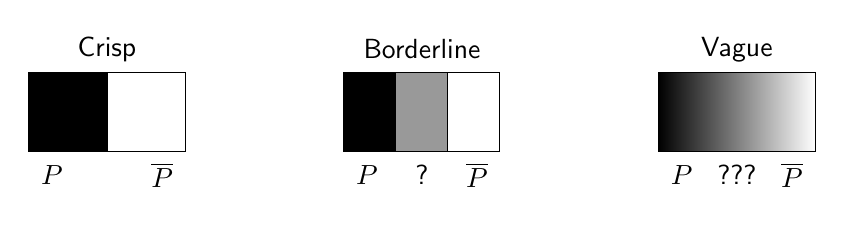
\begin{tikzpicture}[]

        % no borderline

        \node at (1,1.3) {Crisp};

        \draw[fill=black] (0,0) rectangle +(1,1);

        \draw[fill=white] (1,0) rectangle +(1,1);

        \node at (0.3,-0.3) {$P$};

        \node at (1.7,-0.3) {$\overline{P}$};

        % 1 borderline

        \node at (5,1.3) {Borderline};
  
        \draw[fill=black] (4,0) rectangle +(.66,1);

        \draw[fill=black!40] (4.66,0) rectangle +(.66,1);

        \draw[fill=white] (5.32,0) rectangle +(.66,1);

        \node at (4.3,-0.3) {$P$};

        \node at (5,-0.3) {?};

        \node at (5.7,-0.3) {$\overline{P}$};

        % Vague

        \node at (9,1.3) {Vague};

        \shade[left color=black,right color=white,draw=black] (8,0)
        rectangle +(2,1);

        \node at (8.3,-0.3) {$P$};

        \node at (9,-0.3) {???};

        \node at (9.7,-0.3) {$\overline{P}$};

      \end{tikzpicture}
    \end{center}

  

  
  \begin{block}{Vague strategies}
    \vspace*{-0.25cm}
    \begin{center}
      \includegraphics[]{//Users/micha/Desktop/data/svn/stoch_choice_vague/text/post_proc_lenls2010/plot_QRE}
    \end{center}
  \end{block}

\end{frame}



\begin{frame}

\frametitle{Problem: vagueness is irrational / unstable in sim-max games}

\begin{itemize}
\item rational players will never prefer a vague language over a
  precise one
\item vague languages can never be evolutionarily stable
\end{itemize}

  \slideFN{\citep{Lipman2009:Why-is-Language}}

\end{frame}

\begin{frame}
  \frametitle{Possible solutions}

  \begin{block}{Re-rationalizing vagueness}
    vague language could useful after all:
    \vspace*{-0.3cm}
    \begin{multicols}{2}
      \begin{itemize}
      \item flexibility
      \item indirectness
      \item less effortful
      \item \dots
      \end{itemize}
    \end{multicols}
    \hfill     
    \mygray{\footnotesize{\citep[e.g.][]{Jaegherde-Jaegher2003:A-Game-Theoreti,Jaegherde-JaegherRooijvan-Rooij2010:Strategic-Vague,BlumeBoard2013:Intentional-Vag}}}
  \end{block}

   \medskip

    \begin{block}{De-rationalizing vagueness}
    language is vague because
    \begin{itemize}
    \item there are natural limits to human cognitive abilities\\
      \mygray{$\leadsto$ perfectly crisp language is impossible}
    \item there is usually no need for a more precise language\\
      \mygray{$\leadsto$ vague language is good enough}
    \end{itemize}
  \end{block}
      \hfill
    \mygray{\footnotesize{\citep[e.g.][]{FrankeJager2010:Vagueness-Signa,OConnor2013:The-Evolution-o,Correia2013:The-Bivalent-Tr}}}

\end{frame}



\section{Imitation of success}
\subsection{dummy}

\begin{frame}
  \frametitle{Imitation of successes}
  
  \begin{block}{Idea}
  \begin{itemize}
  \item huge, virtually infinite population
  \item each agent holds a pure sender and a pure receiver stratey
  \item every now and then, agent $i$ get a revision opportunity:
    \begin{itemize}
    \item $i$ observes what some agent $j$ sends $\messg$ at choice point $\state$
    \item $i$ henceforth sends $\messg$ in $\state$ with probability $\EU(\messg, \state, \Rstrat)$
    \end{itemize}
  \end{itemize}
\end{block}

\end{frame}

\begin{frame}
  \frametitle{Deriving the replicator dynamic (1/2)}
  
  \begin{block}{In-/Outflow}
    \begin{align*}
  P(\messg' \rightarrow m, \state) & = \sum_{\messg'} \underbrace{\Sstrat(\messg' \probbar
    \state)}_{\text{learner plays $\messg'$}} \cdot
  \underbrace{\Sstrat(\messg \probbar \state)}_{\text{teacher plays $\messg$}} \cdot
  \underbrace{\EU(\messg, \state, \Rstrat)}_{\text{EU teacher choice}} \\
  P(\messg \rightarrow m', \state) & = \sum_{\messg'} \underbrace{\Sstrat(\messg \probbar
    \state)}_{\text{learner plays $\messg$}} \cdot
  \underbrace{\Sstrat(\messg' \probbar \state)}_{\text{teacher plays $\messg'$}} \cdot
  \underbrace{\EU(\messg', \state, \Rstrat)}_{\text{EU teacher choice}}
\end{align*}

  \end{block}

  \begin{block}{Expected change (continuous)}
    \begin{align*}
  \dot{\Sstrat}(\messg \probbar \state) & = P(\messg' \rightarrow m, \state) - P(\messg
  \rightarrow m', \state) \\
& = \underbrace{\Sstrat(\messg \probbar
    \state)}_{\text{frequency of $\messg$ at $\state$}}  \Big ( \underbrace{\EU(\messg,
  \state, \Rstrat)}_{\text{EU of $\messg$ at $\state$}} -   \underbrace{\sum_{\messg'}
      \Sstrat(\messg' \probbar \state) \cdot \EU(\messg',\state,\Rstrat)}_{\text{average
      EU at choice point $\state$}} \Big )
\end{align*}

  \end{block}
  
\end{frame}

\begin{frame}
  \frametitle{Deriving the replicator dynamic (1/2)}

  derivation by infinitesimally small update steps

   \begin{align*}
    \dot{\sigma}(\messg \probbar \state) & = \sigma'(\messg \probbar \state) - \sigma(\messg
    \probbar \state)\\ 
    & = \frac{\Sstrat(\messg \probbar
    \state)  \myts \EU(\messg,\state,\Rstrat)}{\sum_{\messg'}\Sstrat(\messg' \probbar
    \state)  \myts \EU(\messg,\state,\Rstrat)} - \sigma(\messg
      \probbar \state) \\
    & = \frac{\Sstrat(\messg \probbar
    \state)  \myts \EU(\messg,\state,\Rstrat) - \Sstrat(\messg \probbar \state) \sum_{\messg'}\Sstrat(\messg' \probbar
    \state)  \myts \EU(\messg,\state,\Rstrat) }{\sum_{\messg'}\Sstrat(\messg' \probbar
    \state)  \myts \EU(\messg,\state,\Rstrat)}
  \end{align*}

  
  \bigskip

  drop denominator to retrieve continuous-time formulation

\end{frame}

\section{Imprecise imitation}
\subsection{dummy}

\begin{frame}
  \frametitle{Perceptual imprecision}
  
  \begin{itemize}
  \item[] \mymark{now:} states are confused proportional to their similarity
    \vspace*{-0.25cm}
    \begin{multicols}{3}
      \begin{itemize}
      \item[] during play
      \item[] during imitation
        \item[]
      \end{itemize}
    \end{multicols}

  \end{itemize}


  \begin{block}{source of imprecision}
    \begin{enumerate}
    \item \emph{observation noise:} whenever a state $\mystate{a}$ actually occurs, the
      probability that an agent observes it as $\mystate{o}$ is
      $P_o(\mystate{o} \probbar \mystate{a})$;
    \item \emph{realization noise:} whenever an agent intends to realize interpretation
      $\mystate{i}$, the probability that $\mystate{r}$ is realized is
      $P_r(\mystate{r} \probbar \mystate{o})$.
    \end{enumerate}
  \end{block}


\end{frame}

\begin{frame}
  \frametitle{Playing with imprecision}

    \begin{tikzpicture}[->,auto,semithick,>=stealth',every label/.style={gray},node distance=1.9cm]

  \node (1) {};
  \node (2) [right of=1,label=below:$P_a(\mystate{a})$] {$\mystate{a} \in \States$};
  \node (2') [right of=2,label=below:$P_o(\mystate{o} \probbar \mystate{a})$] {$\mystate{o} \in \States$};
  \node (3) [right of=2',label=below:$\Sstrat(\messg \probbar \mystate{o})$] {$\messg \in \Messgs$};
  \node (4) [right of=3,label=below:$\Rstrat(\mystate{i} \probbar \messg)$] {$\mystate{i} \in \States$};
  \node (4') [right of=4,label=below:$P_r(\mystate{r} \probbar \mystate{i})$] {$\mystate{r} \in \States$};

  \path
    (1) edge node {N} (2)
    (2) edge node {} (2')
    (2') edge node {S} (3)
    (3) edge node {R} (4)
    (4) edge node {} (4');

  \end{tikzpicture}

  \pause

\begin{align*}
  P_{\overline{o}}(\mystate{a} \probbar \mystate{o}) & \propto P_a(\mystate{a}) P_o(\mystate{o}
    \probbar \mystate{a}) \\
    P_{\Sstrat}(\messg \probbar \mystate{a}) & = \sum_{\mystate{o}} P_o(\mystate{o} \probbar
  \mystate{a}) \Sstrat(\messg \probbar \mystate{o}) \\
   P_{\overline{\Sstrat}}(\mystate{a} \probbar \messg) & \propto P_a(\mystate{a})
  P_{\Sstrat}(\messg \probbar \mystate{a}) \\
  P_{\Rstrat}(\mystate{r} \probbar \messg) & = \sum_{\mystate{i}} P_r(\mystate{r} \ \probbar
  \mystate{i}) \Rstrat(\mystate{i} \probbar \messg)\\
  P_o(\messg \probbar \mystate{o}) & = \sum_{\mystate{a}} P_{\overline{o}}(\mystate{a}
  \probbar \mystate{o}) \myts P_{\Sstrat}(\messg \probbar \mystate{a}) \\
  P_o(\mystate{o} \probbar \messg) & = \sum_{\mystate{r}} P_o(\mystate{o} \probbar \mystate{r})
  \myts P_{\Rstrat}(\mystate{r} \probbar \messg)
\end{align*}

\end{frame}

\begin{frame}
  \frametitle{Expected utility / average fitness}
  \framesubtitle{at a choice point}

\begin{align*}
  \EU^*(\messg , \mystate{o}, \Rstrat) & = \sum_{\mystate{a}} P_{\overline{o}}(\mystate{a}
  \probbar \mystate{o}) \sum_{\mystate{r}} P_\Rstrat(\mystate{r} \probbar
  \messg) \utils(\mystate{a}, \mystate{r}) \\
  \EU^*(\mystate{i}, \messg, \Sstrat) & = \sum_{\mystate{a}} P_{\overline{\Sstrat}}(\mystate{a}
  \probbar \messg) \sum_{\mystate{r}} P_{r}(\mystate{r} \probbar \mystate{i})
  \utils(\mystate{a}, \mystate{r})
\end{align*}

\end{frame}


\begin{frame}
  \frametitle{Imprecise imitation dynamic}
  
  \begin{align*}
  \Sstrat'(\messg \probbar \state) & \propto P_o(\messg \probbar \state) \myts \EU^*(\messg,
  \state, \Rstrat)\\ 
  \Rstrat'(\state \probbar \messg) & \propto P_o(\state \probbar \messg)
  \myts \EU^*(\state, \messg, \Sstrat)
\end{align*}

\bigskip

\begin{block}{Replicator dynamic}
  \begin{align*}
    \Sstrat'(\messg \probbar \state) & \propto \Sstrat(\messg \probbar \state) \myts
    \EU(\messg, \state,\Rstrat) \\ \Rstrat'(\state \probbar \messg) & \propto \Rstrat(\state
    \probbar \messg) \myts \EU(\state, \messg,\Sstrat)
  \end{align*}
\end{block}




\end{frame}




\miniframesoff

\begin{frame}[plain]
  \frametitle{Summary}
  
  \begin{enumerate}
  \item meaning evolution without predefined states
  \item co-evolution of categories and meanings \medskip
  \item sim-max games
    \begin{itemize}
    \item[] replicator dynamics in behavioral strategies\medskip 
    \end{itemize}
  \item vagueness in meaning
  \end{enumerate}
\end{frame}

%%%%%%%%%%%%%%%%%%%% 

\miniframesoff

\setbeamercolor{normal text}{fg=black}
\setbeamercolor{structure}{fg=black}
\setbeamercolor{frame title}{fg=mycol}

\renewcommand*{\bibfont}{\footnotesize}

\begin{frame}[plain]
  \large{\color{mycol}{References}}
  \vspace*{-0.45cm}
  \begin{multicols}{2}
    \begin{tiny}
      \printbibliography[heading=subbibliography]
    \end{tiny}
  \end{multicols}

\end{frame}



\end{document}


